\documentclass[../main.tex]{subfiles}




\begin{document}


\chapter{Aplicacions de l'homologia}



\section{Homologia reduïda}

En aquest apartat s'introdueix l'homologia reduïda d'un espai topològic. Aquesta homologia és una variant de l'homologia singular que permetrà formular amb més concisió alguns dels càlculs i raonaments dels propers apartats. No és res de concepte, sinó més aviat una qüestió de notació.

Sigui $X$ un espai topològic i $*$ l'espai topològic amb només un element. Considerem l'aplicació constant $\varepsilon:X\rightrightarrows *$.
\begin{defi}
[Homologia reduïda]\index{Homologia reduïda} Es defineix l'homologia reduïda de $X$ com
\begin{equation}
    \notag
    \Tilde{H}_p(X) = \ker\left[\varepsilon_p:H_p(X)\rightarrow H_p(*)\right]
\end{equation}
amb $\Tilde{H}_0(X) = \ker(\varepsilon_p:H_p(X)\rightarrow \mathbb{Z})$ i $\Tilde{H}_p(X) = H_p(X)$ si $p\geq 1$.
\end{defi}

\begin{prop}
Algunes propietats de l'homologia reduïda són
\begin{enumerate}[(i)]
    \item Si $X$ és contràctil, aleshores $\Tilde{H}_\bullet(X) = 0$.
    \item Si $X$ té $r$ components arc-connexes,
    \begin{equation}
        \notag
        \Tilde{H}_0(X)\cong\mathbb{Z}^{\oplus r-1}
    \end{equation}
    \item Si $f:X\rightarrow Y$ és contínua, indueix $\Tilde{f}_p:\Tilde{H}_p(X)\longrightarrow \Tilde{H}_p(Y)$.
    \item Si $f,g:X\rightarrow Y$ són homòtopes, indueixen la mateixa aplicació en homologies reduïdes.
    \item Si $X$ és un espai topològic, $A\subset X$, tenim una successió exacta llarga
    \begin{equation}
        \notag
        \cdots \rightarrow \Tilde{H}_p(A)\rightarrow \Tilde{H}_p(X)\rightarrow H_p(X,A)\rightarrow \Tilde{H}_{p-1}(A)\rightarrow\cdots
    \end{equation}
\end{enumerate}
\end{prop}
\begin{proof}
Com l'homologia reduïda coincideix amb l'homologia en dimensions més grans que $0$ i la diferència pels grups $H_0$ és prou simple, resulta immediat provar que l'homologia reduïda té propietats anàlogues a les de l'homologia singular.
\end{proof}


\begin{ej}
\begin{enumerate}
    \item Si $X$ té $r$ components arc-connexes, amb $r\geq 1$, llavors $\Tilde{H}_0(X)\cong \mathbb{Z}^{\oplus r+1}$ i, en particular, $X$ és arc-connex si, i només si, $\Tilde{H}_0(X)=0$.
    \item Si $X$ és un espai topològic contràctil, $\Tilde{H}_\bullet(X)=0$ i en particular $\Tilde{H}_\bullet(\mathbb{R}^n)=0$.
\end{enumerate}
\end{ej}

\begin{prop}
Sigui $X$ un espai topològic i $U$ i $V$ oberts de $X$ tals que $X = U\cup V$. Si $U\cap V\not=\emptyset$ llavors les inclusions naturals indueixen una successió exacta
\begin{equation}
    \notag
    \cdots\rightarrow\Tilde{H}_p(U\cap V)\rightarrow \Tilde{H}_p(U)\oplus \Tilde{H}_p(V)\rightarrow \Tilde{H}_p(X)\rightarrow \Tilde{H}_{p-1}(U\cap V)\rightarrow\cdots
\end{equation}
que s'anomena successió exacta de Mayer-Vietoris en homologia reduïda.
\end{prop}
\begin{proof}
Segons el que hem comentat i la definició de homologia reduïda aquesta successió és exactament la mateixa que la successió usual de Mayer-Vietoris que ja vam veure, llevat dels termes de grau zero. 

Considerem els termes de grau zero i el següent diagrama commutatiu
\begin{equation}
    \notag
    \xymatrix{
    & \vdots \ar[d] & \vdots \ar[d] & \vdots \ar[d] & \\
    0\ar[r] & \Tilde{H}_1(X)\ar[r]\ar[d] & H_1(X)\ar[r]\ar[d] & 0\ar[r]\ar[d] & 0 \\
    0 \ar[r] & \Tilde{H}_0(U\cap V)\ar[r]\ar[d] & H_0(U\cap V)\ar[r]\ar[d] & \mathbb{Z}\ar[r]\ar[d] & 0\\
    0 \ar[r] & \Tilde{H}_0(U)\oplus \Tilde{H}_0(V)\ar[r]\ar[d] & H_0(U)\oplus H_0(V)\ar[d]\ar[r]& \mathbb{Z}\oplus \mathbb{Z}\ar[r]\ar[d] & 0 \\
    0 \ar[r] & \Tilde{H}_0(X)\ar[r]\ar[d] & H_0(X)\ar[r]\ar[d] & \mathbb{Z}\ar[r]\ar[d] & 0 \\
    & 0 & 0 & 0 &
    }
\end{equation}
que té files exactes, perquè en ser no buits tots els espais que intervenen, els morfismes $H_0(*)\rightarrow \mathbb{Z}$ són exhaustius. Anomenem $K_\bullet, M_\bullet$ i $L_\bullet$ els complexos formats per la primera, segona i tercera columna respectivament, de manera que el diagrama anterior correspon a la successió exacta de complexos
\begin{equation}
    \notag
    0\longrightarrow K_\bullet\longrightarrow M_\bullet\longrightarrow L_\bullet\longrightarrow 0.
\end{equation}
$M_\bullet$ és la successió exacta de Mayer-Vietoris usual, i per tant és un complex exacte. El complex $L_\bullet$ és exacte trivialment, per tant, $H_\bullet(M_\bullet)=0$ i $H_\bullet(L_\bullet) = 0$. Així, si considerem la successió exacta llarga d'homologia associada
\begin{equation}
    \notag
    \cdots\longrightarrow H_{p+1}(L_\bullet)\longrightarrow H_p(K_\bullet)\longrightarrow H_p(M_\bullet)\longrightarrow H_p(L_\bullet)\longrightarrow\cdots
\end{equation}
en resulta immediatament que $K_\bullet$ és un complex exacte i per tant, que la successió de Mayer-Vietoris en homologia reduïda és exacta.
\end{proof}

\section{Teorema de no separació}

Denotarem $I = [0,1]$, $I^r = [0,1]\times\overset{r)}{\cdots}\times [0,1]$ i $\mathbb{B}^r=\{x\in\mathbb{R}^r\;:\;\sum_{i=1}^r x_i^r\leq 1\}$.

\begin{nota}
$I^r$ és homeomorf a $\mathbb{B}^r$.
\end{nota}
\begin{proof}
Exercici. Ja es va fer en el seu moment.
\end{proof}

\begin{defi}
Si $X$ és un espai topològic, $\varphi:I^r\rightarrow X$ contínua i tal que $I^r\rightarrow \varphi(I^r)$ és homeomorf. Direm que $\varphi(I^r)$ és una bola topològica de dimensió $r$ en $X$.
\end{defi}

\begin{ter}[No-separació]
Sigui $e^r$ una bola topològica en $\mathbb{S}^n=\{x\in\mathbb{R}^{n+1}\;:\;\sum_{i=1}^r x_i^2=1\}$. Aleshores $\mathbb{S}^n\setminus e^r\not=\emptyset$ i a més,
\begin{equation}
    \notag
    \Tilde{H}_p(\mathbb{S}^n\setminus e^r) =0\quad\forall p\geq 0
\end{equation}
\end{ter}
\begin{proof}
Observem en primer lloc que $\mathbb{S}^n\setminus e^r$ és no buit, ja que en cas contrari tindríem $\mathbb{S}^n = e^r$ el que és absurd perquè $e^r$ és contràctil i $\mathbb{S}^n$ no.

Provem ara per inducció sobre $r$ que es verifica $\Tilde{H}_\bullet(\mathbb{S}^n\setminus e^r) = 0$. Per $r = 0$, $e^0$ és només un punt, i per tant $\mathbb{S}^n\setminus e^0$ és homeomorf a $\mathbb{R}^n$, d'on se segueix que
\begin{equation}
    \notag
    \Tilde{H}_\bullet(\mathbb{S}^n\setminus e^0)\cong \Tilde{H}_\bullet(\mathbb{R}^n) = 0.
\end{equation}

Fem el pas d'inducció. Suposem cert el teorema per boles topològiques de dimensió $r-1$ i provem-lo per una bola de dimensió $r$, $e^r=\varphi(I^r)$. Sigui $[z]\in H_p(\mathbb{S}^n\setminus e^r)$ una classe d'homologia. Volem provar que $[z] = 0$, és a dir, que $z$ és una vora a $\mathbb{S}^n\setminus e^r$. Dividim la prova en dues etapes:
\begin{enumerate}
    \item Considerem les boles de dimensió $r$ de $\mathbb{S}^n$ donades per
    \begin{equation}
        \notag
        e_1^r = \varphi(I^{r-1}\times[0,1/2])
    \end{equation}
    \begin{equation}
        \notag
        e_2^r = \varphi(I^{r-1}\times[1/2,1])
    \end{equation}
    i la bola de dimensió $r-1$
    \begin{equation}
        \notag
        e^{r-1} = \varphi(I^{r-1}\times\{1/2\})
    \end{equation}
    que per entendre-ho millor enganxo la figura \ref{fig:celleser} dels apunts. 
    \begin{figure}
        \centering
        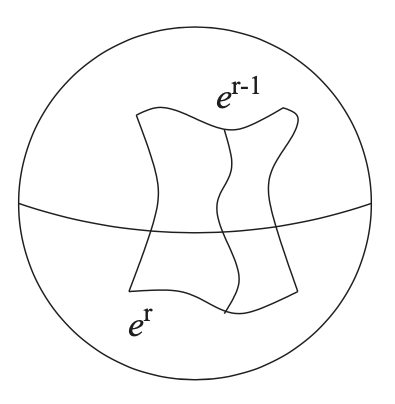
\includegraphics[scale = 0.25]{pictures/celleser.png}
        \caption{Les cel·les $e^r$ i $e^{r-1}$.}
        \label{fig:celleser}
    \end{figure}
    
    Si $[z]\not=0$ aleshores al menys per un dels morfismes en homologia induits per les inclusions
    \begin{equation}
        \notag
        \mathbb{S}^n\setminus e^r\hookrightarrow \mathbb{S}^n\setminus e_i^r,\quad i=1,2
    \end{equation}
    la imatge de $[z]$ és no nul·la. En efecte, notem $U = \mathbb{S}^n\setminus e_1^r$ i $V= \mathbb{S}^n\setminus e_2^r$. Observem que 
    \begin{equation}
        \notag
        U\cap V = \mathbb{S}^n\setminus e^r\quad \text{i}\quad U\cup V = \mathbb{S}^n\setminus e^{r-1}.
    \end{equation}
    En particular, $U\cap V\not=\emptyset$ i per tant podem utilitzar la definició de Mayer-Vietoris en homologia reduïda, corresponent a aquest recobriment
    \begin{equation}
        \notag
        \Tilde{H}_{p+1}(\mathbb{S}^n\setminus e^{r-1})\rightarrow \Tilde{H}_p(\mathbb{S}^n\setminus e^r)\rightarrow \Tilde{H}_p(\mathbb{S}^n\setminus e_1^r)\oplus \Tilde{H}_p(\mathbb{S}^n\setminus e_2^r)\rightarrow\Tilde{H}_p(\mathbb{S}^n\setminus e^{r-1})
    \end{equation}
    Per hipòtesi d'inducció $\Tilde{H}_\bullet(\mathbb{S}^n\setminus e^{r-1}) =0$, i per tant resulten isomorfismes
    \begin{equation}
        \notag
        \Tilde{H}_p(\mathbb{S}^n\setminus e^r)\cong \Tilde{H}_p(\mathbb{S}^n\setminus e_1^r)\oplus \Tilde{H}_p(\mathbb{S}^n\setminus e_2^r),
    \end{equation}
    el que prova que $[z]$ ha de tenir una imatge no nul·la per alguna de les inclusions esmentades.
    
    \item Provem ara que no hi ha classes $[z]$ diferents de zero. Suposem que existeix $[z]\not=0$. Pel que acabem de provar en la primera etapa, la classe de $[z]$ serà no nul·la a $\mathbb{S}^n\setminus e_i^r$ per a $i = 1$ o $i=2$. Suposem que $[z]\not=0$ en $\mathbb{S}^n\setminus e_1^r$. Podem repetir el procés a l'interval $[0,1/2]$, és a dir, considerar les cel·les $\varphi(I^{r-1}\times[0,1/4])$ i $\varphi(I^{r-1}\times[1/4,1/2])$, i concloure que la imatge de $[z]$ en el complementari d'alguna d'aquestes boles és no nul·la. Iterant la primera etapa s'obté una successió d'intervals encaixats
    \begin{equation}
        \notag
        \cdots [a_2,b_2]\subset[a_1,b_1]\subset[0,1]
    \end{equation}
    amb $b_i-a_i = (1/2)^{i}$ i tals que la imatge de $[z]$ a $\Tilde{H}_p(\mathbb{S}^n\setminus \varphi(I^{r-1}\times[a_i,b_i])$ és diferent de zero per a tot $i$. Com la longitud dels intervals encaixats $[a_i,b_i]$ tendeix a zero, la intersecció de tots ells serà un punt. Notem $\{c\}=\cap_i[a_i,b_i]$ i sigui
    \begin{equation}
        \notag
        e^{r-1} = \varphi(I^{r-1}\times\{c\}) = \cap_i\varphi(I^{r-1}\times[a_i,b_i])
    \end{equation}
    de forma que els oberts $U_i = \mathbb{S}^n\setminus\varphi(I^{r-1}\times[a_i,b_i])$ formen un recobriment obert de $\mathbb{S}^n\setminus e^{r-1}$:
    \begin{equation}
        \notag
        \mathbb{S}^n\setminus e^{r-1} = \cup_i(\mathbb{S}^n\setminus\varphi(I^{r-1}\times[a_i,b_i]).
    \end{equation}
    Per hipòtesi d'inducció, $\Tilde{H}_p(\mathbb{S}^n\setminus e^{r-1}) = 0$, per a tot $p\geq 0$, per tant, $z = \partial w$ en el complementari de $e^{r-1}$. Sigui $w = \sum_j\lambda_j\sigma_j$, on $\sigma_j$ són $(p+1)$-símplexs singulars, el suport de la cadena $w$
    \begin{equation}
        \notag
        \mathrm{sup}w = \cup_j\sigma_j(\Delta^{p+1})
    \end{equation}
    és compacte, i per tant del recobriment de $\mathrm{sup}w$ induït pels oberts $U_i$ se'n pot extreure un subrecobriment finit. Però, com $U_i\subseteq U_{i+1}$, això significa que existirà un $j$ de forma que
    \begin{equation}
        \notag
        \mathrm{sup}w\subseteq U_j =\mathbb{S}^n\setminus\varphi(I^{r-1}\times[a_j,b_j]),
    \end{equation}
    és a dir, $[z]$ és zero a $\Tilde{H}_p(\mathbb{S}^n\setminus\varphi(I^{r-1}\times[a_j,b_j]))$, el que és contradictori amb l'elecció dels intervals $[a_j,b_j]$.
\end{enumerate}
\end{proof}

El teorema de no separació que acabem de veure dona l'anul·lació de l'homologia reduïda del complementari d'una bola topològica de $\mathbb{S}^n$, i sembla natural preguntar-se si aquest complementari és contràctil. La resposta és negativa, encara que no és fàcil donar un contraexemple.

\section{El teorema de separació de Jordan-Brouwer}

Recordem que una corba de Jordan del pla $\mathbb{R}^2$ és, per definició, una corba $\alpha:[0,1]\rightarrow \mathbb{R}$ contínua i tal que $\alpha(0) = \alpha(1)$ i és injectiva. Equivalentment, una corba de Jordan és una aplicació contínua i injectiva $\Tilde{\alpha}:\mathbb{S}^1\rightarrow\mathbb{R}^2$. El clàssic teorema de la corba de Jordan s'enuncia com segueix: \textit{el complementari d'una corba de Jordan en el pla té exactament dues components connexes, una d'elles acotada i l'altra no, que la tenen per frontera comú}. 

L'objectiu d'aquest apartat és provar aquest teorema i, de fet, provarem una generalització d'aquest resultat en qualsevol dimensió, en la que l'ingredient essencial de la demostració és el teorema de no separació de l'apartat anterior. Per fer-ho, ens serà més còmode estudiar el complementari d'una corba de Jordan a $\mathbb{S}^2$ en lloc de $\mathbb{R}^2$, i en general a $\mathbb{S}^n$. De fet, és equivalent estudiar el nombre de components connexes del complementari en un i altre cas: si $\varphi:\mathbb{S}^r\rightarrow\mathbb{R}^n$ és una aplicació contínua, $\varphi(\mathbb{s}^r)$ és un compacte i per tant $\mathbb{R}^n\setminus\varphi(\mathbb{S}^r)$ té una única component no acotada, i així, el nombre de components connexes de $\mathbb{R}^n\setminus\varphi(\mathbb{S}^r)$ i $\mathbb{S}^n\setminus\varphi(\mathbb{S}^r)$ és el mateix.

\begin{ter}
[Separació]\index{Teorema de separació de Jordan-Brouwer}\label{ter:separaciojordanbrouwer} Sigui $\varphi:\mathbb{S}^r\rightarrow\mathbb{S}^n$ una aplicació que és un homeomorfisme de $\mathbb{S}^r$ amb la seva imatge $s^r:=\varphi(\mathbb{S}^r)$. Aleshores:
\begin{enumerate}
    \item Si $s^r = \mathbb{S}^n$, llavors $r = n$ i $\varphi:\mathbb{S}^n\rightarrow\mathbb{S}^n$ és un homeomorfisme.
    \item Si $s^r\not=\mathbb{S}^n$, llavors
    \begin{equation}
        \notag
        \Tilde{H}_p(\mathbb{S}^n\setminus s^r)\cong\left\{
        \begin{array}{ll}
            \mathbb{Z} & \text{si $p=n-r-1$} \\
            0 & \text{altrament}
        \end{array}
        \right.
    \end{equation}
    i, en particular, $r<n$.
\end{enumerate}
\end{ter}
\begin{proof}
Si $s^r = \mathbb{S}^n$, llavors $\varphi:\mathbb{S}^r\rightarrow\mathbb{S}^n$ és un homeomorfisme, on $\mathbb{S}^r$ i $\mathbb{S}^n$ són varietats topològiques de dimensions $r$ i $n$ respectivament i per tant $r = n$, pel teorema d'invariància de la dimensió.

Suposem ara que $s^r\not=\mathbb{S}^n$. Aleshores $\mathbb{S}^n\setminus s^r\not=\emptyset$ i calcularem l'homologia reduïda $\Tilde{H}_\bullet(\mathbb{S}^n\setminus s^r)$ per inducció sobre $r$.

Si $r = 0$, $s^0$ està formada per dos punts diferents de l'esfera, $s^0 = \{x,y\}$ amb $x\not=y$, i tindrem isomorfismes
\begin{equation}
    \notag
    \Tilde{H}_\bullet(\mathbb{S}^n\setminus\{x,y\})\cong\Tilde{H}_\bullet(\mathbb{R}^n\setminus\{y\})\cong\Tilde{H}_\bullet(\mathbb{S}^{n-1}),
\end{equation}
i per tant
\begin{equation}
    \notag
    \Tilde{H}_p(\mathbb{S}^n\setminus s^0)\cong\left\{
    \begin{array}{ll}
        \mathbb{Z}, & p=n-1, \\
        0 & p\not=n-1
    \end{array}.
    \right.
\end{equation}
Suposem ara cert el resultat per esferes topològiques de dimensió $r-1$. Usarem les notacions següents:
\begin{equation}
    \notag
    E_+^r = \{x\in\mathbb{S}^r\;:\;x_{r+1}\geq 0\},\qquad E_-^r=\{x\in\mathbb{S}^r\;:\;x_{r+1}\leq 0\},
\end{equation}
i direm $\mathbb{S}^{r-1} = E_+^r\cap E_-^r = \{x\in\mathbb{S}^r\;:\;x_{r+1}=0\}$. També anomenarem $e_+^r=\varphi(E_+^r)$, $e_-^r=\varphi(E_-^r)$ i $s^{r-1} = \varphi(\mathbb{S}^{r-1})$. Observem que es tenen les igualtats
\begin{equation}
    \notag
    \begin{array}{rl}
        s^r & = e_+^r\cup e_-^R, \\
        s^{r-1} & = e_+^r\cap e_-^r, \\
        \mathbb{S}^n\setminus s^r & = (\mathbb{S}^n\setminus e_+^r)\cap(\mathbb{S}^n\setminus e_-^r)\not=\emptyset,\\
        \mathbb{S}^n\setminus s^{r-1} & = \mathbb{S}^n\setminus (e_+^r\cap e_-^r) = (\mathbb{S}^n\setminus e_+^r)\cup(\mathbb{S}^n\setminus e_-^r).
    \end{array}
\end{equation}
La successió exacta de Mayer-Vietoris en homologia reduïda associada és
\begin{equation}
    \notag
    \cdots \rightarrow \Tilde{H}_{p+1}(\mathbb{S}^n\setminus e_+^r)\oplus\Tilde{H}_{p+1}(\mathbb{S}^n\setminus e_-^r)\rightarrow \Tilde{H}_{p+1}(\mathbb{S}^n\setminus s^{r-1})\rightarrow \Tilde{H}_p(\mathbb{S}^n\setminus s^r)\rightarrow \Tilde{H}_p(\mathbb{S}^n\setminus e_+^r)\oplus\Tilde{H}_p(\mathbb{S}^n\setminus e_-^r)\rightarrow\cdots
\end{equation}
Com $e_+^r$ i $e_-^r$ són $r$-boles topològiques podem aplicar el teorema de no separació i deduir que la successió anterior dóna els isomorfismes
\begin{equation}
    \notag
    \Tilde{H}_{p+1}(\mathbb{S}^n\setminus s^{r-1})\cong\Tilde{H}_p(\mathbb{S}^n\setminus s^r),
\end{equation}
el que permet aplicar la hipòtesi d'inducció i deduir
\begin{equation}
    \notag
    \Tilde{H}_p(\mathbb{S}^n\setminus s^r)\cong\Tilde{H}_{p+1}(\mathbb{S}^n\setminus s^{r-1})\cong\left\{
    \begin{array}{ll}
        \mathbb{Z}, & p+1=n-(r-1)-1, \\
        0, & p+1\not=n-(r-1)-1.
    \end{array}
    \right.
\end{equation}
Finalment, suposem que $r\geq n$. Aleshores $\Tilde{H}_p(\mathbb{S}^n\setminus s^r)\cong\mathbb{Z}$ si $p = n-r-1\leq -1$ el que és absurd ja que $\Tilde{H}_p(\mathbb{S}^n\setminus s^r) = 0$ si $p<0$.
\end{proof}

\begin{coro}
\label{coro:jordanbrouwer} \begin{enumerate}
    \item Tota $s^{n-1}$ separa $\mathbb{S}^n$ en dues components connexes.
    \item Si $r<n-1$, llavors $\mathbb{S}^n\setminus s^r$ és connex, és a dir, $s^r$ no separa $\mathbb{S}^n$.
\end{enumerate}
\end{coro}
\begin{proof}
\begin{enumerate}
    \item $\Tilde{H}_0(\mathbb{S}^n\setminus s^{n-1})\cong\mathbb{Z}$, per tant $H_0(\mathbb{S}^n\setminus s^{n-1})\cong\mathbb{Z}^2$, i per tant $\mathbb{S}^n\setminus s^{n-1}$ té dues components arc-connexes o connexes.
    \item Si $r\not=n-1$, el teorema dóna $\Tilde{H}_0(\mathbb{S}^n\setminus s^r) = 0$, i per tant $\mathbb{S}^n\setminus s^r$ és connex.
\end{enumerate}
\end{proof}

Podem expressar el resultat anterior dient que $s^r$ separa $\mathbb{S}^n$ en dimensió $n-r-1$. Observem, però, que el teorema de separació no dóna encara el teorema de la corba de Jordan tal i com l'hem comentat al començament d'aquest apartat, ja que cal precisar la relació entre les components de $\mathbb{S}^n\setminus s^{n-1}$ i l'esfera $s^{n-1}$.

\begin{ter}
[Jordan-Brower]\index{Teorema de Jordan-Brouwer}\label{ter:jordanbrouwer} Sigui $s^{n-1}$ una $(n-1)$-esfera topològica en $\mathbb{S}^n$. Aleshores $\mathbb{S}^n\setminus s^{n-1}$ té dues components connexes amb frontera $s^{n-1}$.
\end{ter}
\begin{proof}
Suposem $U,V$ components arc-connexes de $\mathbb{S}^n\setminus s^{n-1}$. Volem veure que $\partial U = s^{n-1}$. Tenim d'una banda $\partial U\subset s^{n-1}$ fàcilment, ja que observem que $\partial U\subset U\cup s^{n-1}$ ja que si no fos així, voldria dir que la frontera de $U$ tindria algun punt de l'altra component arc-connexa, però la frontera de $U$ és $\partial U= \overline{U}\setminus\mathring{U}$ i aleshores si $\partial U\cap V\not=\emptyset$, tindríem que $\overline{U}\cap V\not=\emptyset$ i per tant seria $U\cap V\not=\emptyset$ la qual cosa és absurda.

Hem de veure l'altra inclusió de la frontera, és a dir, $s^{n-1}\subset\overline{U}$. Sigui $x\in s^{n-1}$, sigui $N$ un entorn obert de $x$. Volem veure que $N\cap U\not=\emptyset$. Tenim
\begin{equation}
    \notag
    \varphi:\mathbb{S}^{n-1}\rightarrow s^{n-1}\subset\mathbb{S}^{n}
\end{equation}
homeomorfisme. Sigui $y\in \mathbb{S}^{n-1}$ tal que $\varphi(y)=x$. Sigui $B$ una bola (mètrica) en $\mathbb{S}^{n-1}$, de centre $y$. Sigui $A = \varphi(B)$ i podem suposar que $A\subset N$. Tenim que $\mathbb{S}^{n-1}\setminus B$ és homeomorf a una bola tancada. Si apliquem $\varphi$, tenim que $e^{n-1}:= s^{n-1}\setminus A$ és una $(n-1)$-bola topològica en $\mathbb{S}^n$. Així, si apliquem el teorema de no separació,
\begin{equation}
    \notag
    \Tilde{H_0}(\mathbb{S}^n\setminus e^{n-1}) = 0
\end{equation}
i, per tant, $Z = \mathbb{S}^n\setminus e^{n-1}$ és connex. 
\begin{figure}
    \centering
    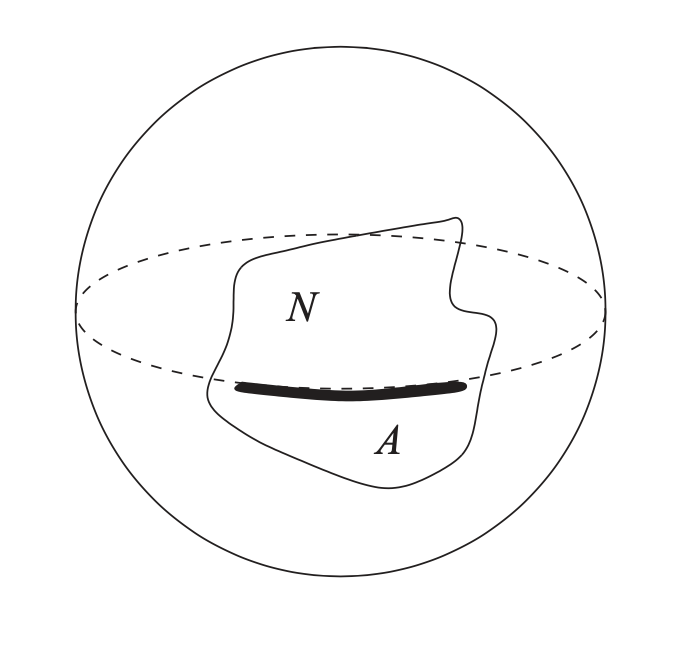
\includegraphics[scale = 0.5]{pictures/jordanbrouwer.png}
    \caption{La bola $A$ i l'entorn $N$.}
    \label{fig:bolaaentornn}
\end{figure}
Com 
\begin{equation}
    \notag
    Z = U\cup V\cup A\subseteq U\cup V\cup N,
\end{equation}
si $N\cap U$ fos buit, aleshores $U\cap(V\cup N)$ també ho seria, i podríem desconnectar $Z$ en la forma
\begin{equation}
    \notag
    Z=(Z\cap U)\cup(Z\cap(V\cup N)),
\end{equation}
el que és absurd perquè $Z$ és connex. Així doncs, $N\cap U\not=\emptyset$.
\end{proof}

Ara ja per fi podem demostrar el teorema de la Corba de Jordan, que era l'objectiu d'aquests apartats. Primer repeteixo en forma de definició què era una corba de Jordan.

\begin{defi}
[Corba de Jordan]\index{Corba de Jordan} Una \textit{corba de Jordan} és la imatge d'una aplicació $\mathbb{S}^1\rightarrow \mathbb{R}^2$ contínua i injectiva.
\end{defi}

\begin{ter}
[Corba de Jordan]\index{Teorema de la Corba de Jordan} Sigui $C\subset\mathbb{R}^2$ una corba de Jordan. Aleshores $\mathbb{R}^2\setminus C$ té exactament dues components connexes, una fitada i l'altra no, i totes dues tenen com a frontera la corba $C$.
\end{ter}
\begin{proof}
Sigui $\mathbb{S}^1\overset{\alpha}{\longrightarrow}\mathbb{R}^2$ tal que $\alpha(\mathbb{S}^1)$ és corba de Jordan. Considerem la projecció estereogràfica $\pi_e^{-1}$ i tenim
\begin{equation}
    \notag
    \mathbb{S}^1\overset{\alpha}{\longrightarrow}\mathbb{R}^2\overset{\pi_e^{-1}}{\longrightarrow}\mathbb{S}^2\setminus\{p\}\subset\mathbb{S}^2
\end{equation}
Tenim que $\alpha';\mathbb{S}^1\rightarrow\mathbb{S}^2$ i $\mathbb{S}^1\cong\alpha(\mathbb{S}^1)$ per tant $\mathbb{S}^2\setminus\alpha(\mathbb{S}^1)$ té dues components connexes i amb frontera $\alpha(\mathbb{S}^1)$ pel teorema que acabem de veure (\ref{ter:jordanbrouwer}). 
\end{proof}

Com a comentari, entenem què diu aquest teorema. Ens ho podem imaginar en $\mathbb{R}^2$ i aleshores pillem una bola $\mathbb{S}^2$ traient-li el punt $p$ que sigui el pol nord. Aleshores la projecció estereogràfica fa que $\mathbb{R}^2\simeq \mathbb{S}^2\setminus\{p\}$ i llavors, de les dues components connexes que té el complementari, una d'elles contindrà $p$ i l'altra no. Si passem la que conté $p$, via l'homeomorfisme $\pi_e^{-1}$ (projecció estereogràfica) a $\mathbb{R}^2$, aleshores obtenim una component que no està fitada i la component que no contingui $p$, via la projecció estereogràfica, ens dona una component connexa fitada en $\mathbb{R}^2$. 




\section{Altres teoremes importants}

Aquest és un teorema que té moltes formulacions equivalents, potser una de les més habituals és la que veurem a continuació. 

\begin{ter}
[Borsuk-Ulam]\index{Teorema de Borsuk-Ulam}\label{ter:borsukulam} Sigui $f:\mathbb{S}^n\rightarrow\mathbb{R}^n$ contínua. Aleshores, existeix un $x\in\mathbb{S}^n$ tal que $f(x) = f(-x)$.
\end{ter}

Ara bé, per conveniència, nosaltres demostrarem la següent formulació.

\begin{ter}
[Borsuk-Ulam]\index{Teorema de Borsuk-Ulam} Sigui $g:\mathbb{S}^n\rightarrow \mathbb{S}^m$ contínua i imparella, és a dir, que per tot $x\in\mathbb{S}^n$ es té $g(x) = -g(-x)$. Llavors, $n\leq m$.
\end{ter}

En el que segueix donarem una demostració del teorema de Borsuk-Ulam que requereix l'homologia amb coeficients en $\mathbb{Z}/2\mathbb{Z}$, mostrant així l'interès de disposar d'aquest tipus de coeficients.

La demostració del teorema es basarà en algunes propietats homològiques del pas al quocient de $\mathbb{S}^n$ per la relació d'equivalència $x\sim-x$, és a dir, de la identificació $\pi:\mathbb{S}^n\rightarrow\mathbb{P}^n$, que resumim en l'enunciat següent:

\begin{prop}
\label{prop:borsuk-ulam} Existeix un morfisme de $\mathbb{Z}/2\mathbb{Z}$-mòduls
\begin{equation}
    \notag
    t_\bullet:H_\bullet(\mathbb{P}^n,\mathbb{Z}/2\mathbb{Z})\longrightarrow H_\bullet(\mathbb{S}^n,\mathbb{Z}/2\mathbb{Z})
\end{equation}
que verifica
\begin{enumerate}[(i)]
    \item La composició
    \begin{equation}
        \notag
        H_\bullet(\mathbb{S}^n,\mathbb{Z}/2\mathbb{Z}\overset{\pi_\bullet}{\longrightarrow} H_\bullet(\mathbb{P}^n,\mathbb{Z}/2\mathbb{Z})\overset{t_\bullet}{\longrightarrow}H_\bullet(\mathbb{S}^n,\mathbb{Z}/2\mathbb{Z})
    \end{equation}
    és nul·la.
    \item Hi ha una successió exacta llarga
    \begin{equation}
        \notag
        H_p(\mathbb{P}^n,\mathbb{Z}/2\mathbb{Z})\overset{t_\bullet}{\longrightarrow} H_p(\mathbb{S}^n,\mathbb{Z}/2\mathbb{Z})\overset{\pi_\bullet}{\longrightarrow} H_p(\mathbb{P}^n,\mathbb{Z}/2\mathbb{Z})\longrightarrow H_{p-1}(\mathbb{P}^n,\mathbb{Z}/2\mathbb{Z})
    \end{equation}
    \item Si $g:\mathbb{S}^n\rightarrow\mathbb{S}^m$ és una aplicació contínua que commuta amb l'aplicació antipodal, i $\Tilde{g}:\mathbb{P}^n\rightarrow\mathbb{P}^m$ denota l'aplicació induïda per $g$, aleshores el diagrama
    \begin{equation}
        \notag
        \xymatrix{
        \ar[r]&H_p(\mathbb{P}^n,\mathbb{Z}/2\mathbb{Z})\ar[r]^{t_\bullet}\ar[d]_{\Tilde{g}_\bullet} & H_p(\mathbb{S}^n)\ar[r]^{\pi_\bullet}\ar[d]_{g_\bullet} & H_p(\mathbb{P}^n,\mathbb{Z}/2\mathbb{Z})\ar[r]\ar[d]_{\Tilde{g}_\bullet} & \\
        \ar[r] & H_p(\mathbb{P}^m,\mathbb{Z}/2\mathbb{Z})\ar[r]^{t_\bullet}& H_p(\mathbb{S}^m,\mathbb{Z}/2\mathbb{Z})\ar[r]^{\pi_\bullet} & H_p(\mathbb{P}^m,\mathbb{Z}/2\mathbb{Z})\ar[r] & 
        }
    \end{equation}
    és un diagrama commutatiu de successions exactes.
\end{enumerate}
\end{prop}
\begin{proof}
Sigui $\mathcal{U}$ un recobriment obert de $\mathbb{S}^n$ tal que si $\mathcal{V}$ és el recobriment de $\mathbb{P}^n$ format pels oberts $V = \pi(U)$ de $\mathbb{P}^n$, amb $U\in\mathcal{U}$, aleshores $\pi$ indueixi homeomorfismes $U\rightarrow V$. Si $\sigma\in S_p(\mathcal{V})$ és un $p$-símplex $\mathcal{V}$-petit, $\sigma(\Delta^p)$ està contingut en un obert $V$ de $\mathcal{V}$, així si $U$ és obert de $\mathcal{U}$ tal que $\pi_{|U}:U\rightarrow V$ és un homeomorfisme, podem considerar el símplex de $\mathbb{S}^n$ definit per $\Tilde{\sigma} = (\pi_{|U})^{-1}\circ\sigma$. Observem que aquest aixecament depèn de l'obert $U$ escollit, però en qualsevol altre obert dóna lloc al mateix aixecament o a $a\ell^n\circ\Tilde{\sigma}$. Definim un morfisme de complexos
\begin{equation}
    \notag
    t_\bullet^{\mathcal{U}}:S_\bullet(\mathcal{V},\mathbb{Z}/2\mathbb{Z})\longrightarrow S_\bullet(\mathcal{U},\mathbb{Z}/2\mathbb{Z})
\end{equation}
que sobre els símplexs singulars val
\begin{equation}
    \notag
    t_\bullet^{\mathcal{U}}(\sigma) = \Tilde{\sigma}+a\ell^n\circ\Tilde{\sigma}.
\end{equation}
Pel teorema de les cadenes petites, $t_\bullet^{\mathcal{U}}$ indueix un morfisme
\begin{equation}
    \notag
    t_\bullet:H_\bullet(\mathbb{P}^n,\mathbb{Z}/2\mathbb{Z})\longrightarrow H_\bullet(\mathbb{S}^n,\mathbb{Z}/2\mathbb{Z})
\end{equation}
a través del següent diagrama
\begin{equation}
    \notag
    \xymatrix{
    H_\bullet(\mathbb{P}^n,\mathbb{Z}/2\mathbb{Z}) & H_\bullet(\mathbb{S}^n,\mathbb{Z}/2\mathbb{Z})\\
    H_\bullet(\mathcal{V},\mathbb{Z}/2\mathbb{Z})\ar[u]^{\cong}\ar[r]^{t_\bullet^{\mathcal{U}}} & H_\bullet(\mathcal{U},\mathbb{Z}/2\mathbb{Z})\ar[u]^{\cong}
    }
\end{equation}
És un exercici comprovar que el morfisme així definit no depèn del recobriment $\mathcal{U}$ escollit.

Per demostrar la primera propietat observem que 
\begin{equation}
    \notag
    (t_\bullet\circ\pi_\bullet)(z) = (1+\deg_2a\ell^n_\bullet)(z)
\end{equation}
per a tot $z\in H_n(\mathbb{S}^n,\mathbb{Z}/2\mathbb{Z})$, i com $\deg_2a\ell = 1$ en homologia amb coeficients en $\mathbb{Z}/2\mathbb{Z}$, per motius que no entenc resulta que $t_\bullet\circ\pi_\bullet = 0$.

Per demostrar la segona propietat és suficient provar que es té la successió exacta de complexos
\begin{equation}
    \notag
    0\longrightarrow S_\bullet(\mathcal{V},\mathbb{Z}/2\mathbb{Z})\overset{t_\bullet}{\longrightarrow}\overset{t_\bullet}{\longrightarrow}S_\bullet(\mathcal{U},\mathbb{Z}/2\mathbb{Z})\overset{\pi_\bullet}{\longrightarrow}S_\bullet(\mathcal{V},\mathbb{Z}/2\mathbb{Z})\longrightarrow 0.
\end{equation}
per la definició de $t_\bullet$, la composició $\pi_\bullet\circ t_\bullet$ correspon a multiplicar per 2, i per tant és zero ja que utilitzem coeficients en $\mathbb{Z}/2\mathbb{Z}$. D'altra banda, si $c$ és una cadena del nucli de $\pi_\bullet$, i $\sigma$ és un símplex de $c$, aleshores $c$ ha de contenir també el símplex $a\ell^n(\sigma)$, i per tant és de la imatge de $t_\bullet$. 

Finalment, la demostració de 1 es deixa com a exercici.
\end{proof}

A continuació farem un càlcul dels grups d'homologia de l'espai $\mathbb{P}^n$ sobre $\mathbb{Z}/2\mathbb{Z}$ i finalment demostrarem el teorema de Borsuk-Ulam.

\begin{coro}
Els grups d'homologia amb coeficients en $\mathbb{Z}/2\mathbb{Z}$ dels espais projectius reals són
\begin{equation}
    \notag
    H_p(\mathbb{P}^n,\mathbb{Z}/2\mathbb{Z})\cong\left\{
    \begin{array}{ll}
        \mathbb{Z}/2\mathbb{Z},  & 0\leq p\leq n, \\
        0, & p>n.
    \end{array}
    \right.
\end{equation}
\end{coro}
\begin{proof}
Si $p>n$, aleshores $H_p(\mathbb{P}^n,\mathbb{Z}/2\mathbb{Z}) = 0$ ja que l'espai projectiu real de dimensió $n$ és un espai triangulable de dimensió $n$.

Considerem ara la successió exacta llarga de la proposició anterior,
\begin{equation}
    \notag
    \rightarrow H_p(\mathbb{P}^n,\mathbb{Z}/2\mathbb{Z})\overset{t_\bullet}{\rightarrow}H_p(\mathbb{S}^n,\mathbb{Z}/2\mathbb{Z})\overset{\pi_\bullet}{\rightarrow}H_p(\mathbb{P}^n,\mathbb{Z}/2\mathbb{Z})\rightarrow H_{p-1}(\mathbb{P}P^n,\mathbb{Z}/2\mathbb{Z})\rightarrow
\end{equation}
Observem que 
\begin{equation}
    \notag
    \pi_\bullet:H_n(\mathbb{S}^n,\mathbb{Z}/2\mathbb{Z})\longrightarrow H_n(\mathbb{P}^n,\mathbb{Z}/2\mathbb{Z}),
\end{equation}
és el morfisme zero, ja que $t_\bullet:H_n(\mathbb{P}^n,\mathbb{Z}/2\mathbb{Z})\rightarrow H_n(\mathbb{S}^n,\mathbb{Z}/2\mathbb{Z})$ és injectiu, com resulta de la successió exacta anterior, mentre que la composició $t_\bullet\circ\pi_\bullet$ és zero segons la proposició que hem vist abans. A més, com $H_p(\mathbb{S}^n,\mathbb{Z}/2\mathbb{Z})=0$, si $0<p<n$, i $\pi_\bullet:H_0(\mathbb{S}^n,\mathbb{Z}/2\mathbb{Z})\rightarrow H_0(\mathbb{P}^n,\mathbb{Z}/2\mathbb{Z})$ és un isomorfisme ja que ambdós espais són connexos, la successió exacta considerada dóna lloc als isomorfismes
\begin{equation}
    \notag
    H_p(\mathbb{P}^n,\mathbb{Z}/2\mathbb{Z})\cong H_{p-1}(\mathbb{P}^n,\mathbb{Z}/2\mathbb{Z}),
\end{equation}
per a tot $1\leq p\leq n$. Així inductivament en resulten els isomorfismes 
\begin{equation}
    \notag
    H_p(\mathbb{P}^n,\mathbb{Z}/2\mathbb{Z})\cong\mathbb{Z}/2\mathbb{Z},\qquad p\leq n,
\end{equation}
d'on se segueix el corol·lari.
\end{proof}

Finalment podem fer ja la demostració del teorema de Borsuk-Ulam. Demostrarem la segona versió, ja que la demostració es basa en això que acabem de veure.

\begin{proof}
[Demostració de Borsuk-Ulam] Sigui $g:\mathbb{S}^n\rightarrow \mathbb{S}^m$ una aplicació equivariant respecte el morfisme antipodal, és a dir, tal que $g(-x) = -g(x)$ per a tot $x\in\mathbb{S}^n$, i suposem que $n>m$. Per la proposició (\ref{prop:borsuk-ulam}) tindrem un diagrama commutatiu de successions exactes
\begin{equation}
        \notag
        \xymatrix{
        \ar[r]&H_p(\mathbb{P}^n,\mathbb{Z}/2\mathbb{Z})\ar[r]^{t_\bullet}\ar[d]_{\Tilde{g}_\bullet} & H_p(\mathbb{S}^n)\ar[r]^{\pi_\bullet}\ar[d]_{g_\bullet} & H_p(\mathbb{P}^n,\mathbb{Z}/2\mathbb{Z})\ar[r]\ar[d]_{\Tilde{g}_\bullet} & \\
        \ar[r] & H_p(\mathbb{P}^m,\mathbb{Z}/2\mathbb{Z})\ar[r]^{t_\bullet}& H_p(\mathbb{S}^m,\mathbb{Z}/2\mathbb{Z})\ar[r]^{\pi_\bullet} & H_p(\mathbb{P}^m,\mathbb{Z}/2\mathbb{Z})\ar[r] & 
        }
\end{equation}

Així, tenint present l'anul·lació de l'homologia de les esferes per sota de la seva dimensió, el diagrama commutatiu de successions exactes llargues dóna lloc, per $1\leq p\leq m$, a diagrames commutatius
\begin{equation}
    \notag
    \xymatrix{
    H_p(\mathbb{P}^n,\mathbb{Z}/2\mathbb{Z})\ar[r]^\sim\ar[d]_{\Tilde{g}_p} & H_{p-1}(\mathbb{P}^n,\mathbb{Z}/2\mathbb{Z})\ar[d]_{\Tilde{g}_{p-1}}\\
    H_p(\mathbb{P}^m,\mathbb{Z}/2\mathbb{Z})\ar[r]^\sim & H_{p-1}(\mathbb{P}^m,\mathbb{Z}/2\mathbb{Z}),
    }
\end{equation}
en el que els morfismes horitzontals són isomorfismes, segons la demostració del corol·lari anterior.

Com els espais projectius són connexos, el morfisme $\Tilde{g}_0:H_0(\mathbb{P}^n,\mathbb{Z}/2\mathbb{Z})\rightarrow H_0(\mathbb{P}^m,\mathbb{Z}/2\mathbb{Z})$ és un isomorfisme, i usant el diagrama anterior es dedueix, inductivament, que els morfismes $\Tilde{g}_p$ són també isomorfismes, per $0\leq p\leq m$.

Per $p = m$ es té també el diagrama commutatiu
\begin{equation}
    \notag
    \xymatrix{
    H_m(\mathbb{P}^n,\mathbb{Z}/2\mathbb{Z})\ar[r]^\sim\ar[d]_{\Tilde{g}_m} & H_{m}(\mathbb{S}^n,\mathbb{Z}/2\mathbb{Z})\ar[d]\\
    H_m(\mathbb{P}^m,\mathbb{Z}/2\mathbb{Z})\ar[r]^\sim & H_{m}(\mathbb{S}^m,\mathbb{Z}/2\mathbb{Z}),
    }
\end{equation}
Com $\Tilde{g}_m$ és un isomorfisme i $H_m(\mathbb{S}^n,\mathbb{Z}/2\mathbb{Z}) = 0$ perquè estem suposant que $n>m$, aquest diagrama és de la forma
\begin{equation}
    \notag
    \xymatrix{
    H_m(\mathbb{P}^n,\mathbb{Z}/2\mathbb{Z})\ar[r]^\sim\ar[d]_{\Tilde{g}_m} & 0\ar[d]\\
    H_m(\mathbb{P}^m,\mathbb{Z}/2\mathbb{Z})\ar[r]^\sim & \mathbb{Z}/2\mathbb{Z},
    }
\end{equation}
el que és absurd.
\end{proof}

Com a conseqüència de la demostració que hem efectuat, podem demostrar també el resultat següent, que és una altra versió del Teorema de Borsuk-Ulam.

\begin{coro}
[Borsuk-Ulam]\index{Teorema de Borsuk-Ulam} Sigui $f:\mathbb{S}^n\rightarrow \mathbb{S}^n$ una aplicació contínua tal que $f(-x) = -f(x)$. Aleshores el grau de $f$ és senar. 
\end{coro}
\begin{proof}
Com $f$ és compatible amb l'aplicació antipodal, $f$ indueix una aplicació contínua $\Tilde{f}:\mathbb{P}^n\rightarrow\mathbb{P}^n$. Segons la demostració anterior del teorema de Borsuk-Ulam, es té un diagrama commutatiu
\begin{equation}
    \notag
    \xymatrix{
    H_n(\mathbb{P}^n,\mathbb{Z}/2\mathbb{Z})\ar[r]^\sim\ar[d]_{\Tilde{f}_n} & H_{n}(\mathbb{S}^n,\mathbb{Z}/2\mathbb{Z})\ar[d]_{f_n}\\
    H_n(\mathbb{P}^n,\mathbb{Z}/2\mathbb{Z})\ar[r]^\sim & H_{n}(\mathbb{S}^n,\mathbb{Z}/2\mathbb{Z}),
    }
\end{equation}
en el que els morfismes horitzontals i $\Tilde{f}_n$ són isomorfismes i, per tant, també ho ha de ser $f_n$. Així doncs, $\deg_2f = 1$, i per tant el grau de $f$ és senar.
\end{proof}










\section{Annex: Grau d'aplicacions entre esferes}

En aquest apartat farem un incís sobre el grau de les aplicacions entre esferes. Això ho faig perquè a classe no es va donar a la teoria, però en canvi hi havia una llista d'exercicis sencera dedicada a aquest apartat. La llista és, de fet, els resultats que veurem a continuació. No obstant això, als apunts que segueixo sí que hi ha un apartat dedicat al grau d'aplicacions entre esferes i és d'aquí d'on trauré la informació.

Recordem primer què era el grau. Sigui $\mathbb{S}^n = \{x\in\mathbb{R}^{n+1}\;:\;\|x\|=1\}$ l'esfera $n$-dimensional, amb $n\geq 0$, com sempre. Tota aplicació ortogonal $f:\mathbb{R}^{n+1}\rightarrow\mathbb{R}^{n+1}$ indueix una aplicació contínua $f:\mathbb{S}^n\rightarrow\mathbb{S}^n$, i d'aquesta forma obtenim un bon nombre d'aplicacions contínues de l'esfera en ella mateixa. Exemples d'aquesta mena d'aplicacions són les rotacions o l'\textit{aplicació antipodal}\index{Aplicació antipodal} definida per
\begin{equation}
    \notag
    \begin{array}{rl}
        a\ell^n: \mathbb{S}^n & \longrightarrow\mathbb{S}^n \\
        x & \longmapsto -x
    \end{array}
\end{equation}
Com podem classificar aquestes aplicacions respecte de la relació d'homotopia? Volem saber, per exemple, si una rotació i l'aplicació antipodal poden ser homòtopes. Per estudiar aquest tipus de qüestió és convenient conèixer l'acció de $f$ en homologia.

En aquest apartat veurem que en el cas de les esferes aquesta acció ve determinada per un cert enter, el grau de $f$, que ja vam definir prèviament molt fora de context (veure índex de paraules). En efecte, $f$ indueix un morfisme
\begin{equation}
    \notag
    f_\bullet:\Tilde{H}_n(\mathbb{S}^n)\longrightarrow\Tilde{H}_n(\mathbb{S}^n),
\end{equation}
i, com $\Tilde{H}_n(\mathbb{S}^n)\cong\mathbb{Z}$, aquest morfisme $f_\bullet$ serà igual a la multiplicació per un enter. A aquest enter l'anomenarem grau:

\begin{defi}
[Grau]\index{Grau}\label{def:grau} Sigui $f:\mathbb{S}^n\rightarrow\mathbb{S}^n$ una aplicació contínua. Es defineix el \textit{grau de $f$} com l'enter $\deg f := z$ tal que
\begin{equation}
    \notag
    f_\bullet:\Tilde{H}_n(\mathbb{S}^n)\longrightarrow \Tilde{H}_n(\mathbb{S}^n)
\end{equation}
és multiplicar per $z$, per a tot $z\in\Tilde{H}_n(\mathbb{S}^n)\cong\mathbb{Z}$. 
\end{defi}

Resumim les propietats més immediates en la següent proposició. 

\begin{prop}
\label{prop:propietatsgrau}
\begin{enumerate}[(1)]
    \item El grau de l'aplicació identitat és 1.
    \item Siguin $f,g:\mathbb{S}^n\rightarrow\mathbb{S}^n$. Si $f$ és homòtopa a $g$, aleshores $\deg f = \deg g$. En particular, si $f$ és homòtopa a una aplicació constant, aleshores $\deg f = 0$.
    \item Siguin $f,g:\mathbb{S}^n\rightarrow \mathbb{S}^n$ aplicacions contínues. Aleshores
    \begin{equation}
        \notag
        \deg(f\circ g) = \deg f\cdotp\deg g
    \end{equation}
    \item Si $f:\mathbb{S}^n\rightarrow\mathbb{S}^n$ és una equivalència homotòpica, aleshores $\deg f = \pm 1$.
\end{enumerate}
\end{prop}
\begin{proof}
Només provaré la 3, ja que les altres són fàcils i es deixen com exercici, i la 3 era un exercici de la llista. És fàcil, donades les igualtats:
\begin{equation}
    \notag
    (f\circ g)_\bullet(z) = f_\bullet(g_\bullet(z)) = f_\bullet(\deg g\cdotp z) = \deg g\cdotp f_\bullet(z) = \deg g\cdotp \deg f\cdotp z
\end{equation}
\end{proof}

El valor del grau de l'aplicació antipodal prova que aquesta no és homòtopa a l'aplicació identitat o a una rotació per a les esferes de dimensió parella, ja que est té el següent resultat:

\begin{prop}\label{prop:grauantipodal}
El grau de l'aplicació antipodal $a\ell^n:\mathbb{S}^n\rightarrow\mathbb{S}^n$ és $(-1)^{n+1}$.
\end{prop}
\begin{proof}
Farem la demostració per inducció sobre $n$. 

Calculem $\deg a\ell^0$. En aquest cas, $\mathbb{S}^0 = \{x,y\}$ amb $x\not=y$ i l'homologia reduïda està generada pel $0$-cicle $[x-y]$ ja que es té
\begin{equation}
    \notag
    H_0(\mathbb{S}^0) = \ker(H_0(\mathbb{S}^0)\cong\mathbb{Z}[x]\oplus \mathbb{Z}[y]\longrightarrow H_0(*))=\mathbb{Z}[x-y].   
\end{equation}
D'altra banda, l'aplicació antipodal intercanvia els punts $x$ i $y$, i per tant
\begin{equation}
    \notag
    a\ell^0_\bullet(x-y) = y-x = -(x-y),
\end{equation}
és a dir, $\deg a\ell^0 = -1$.

Suposem ara cert el resultat per a esferes de dimensió $n-1$ i provem-lo per a esferes de dimensió $n$. Prenem un punt qualsevol $R\in\mathbb{S}^n$ i la seva imatge $T = a\ell^n(R)$ i considerem el recobriment de $\mathbb{S}^n$ format pels oberts
\begin{equation}
    \notag
    U = \mathbb{S}^n\setminus \{R\},\qquad V = \mathbb{S}^n\setminus\{T\}. 
\end{equation}
La intersecció és $U\cap V = \mathbb{S}^n\setminus\{R,T\}$, i és homotòpicament equivalent a l'esfera $\mathbb{S}^{n-1}$. L'aplicació antipodal canvia $U$ per $V$ i, a més, és compatible amb la retracció de $U\cap V$ sobre l'esfera $\mathbb{S}^{n-1}$, induint en aquesta l'aplicació antipodal $a\ell^{n-1}$. Per tant, es té un diagrama commutatiu de successions de Mayer-Vietoris
\begin{equation}
    \notag
    \xymatrix{
    \Tilde{H}_n(U)\oplus\Tilde{H}_n(V)\ar[d]_{a\ell^n_\bullet}\ar[r]^p & \Tilde{H}_n(\mathbb{S}^n)\ar[d]_{a\ell^n_\bullet}\ar[r]^{\delta} & \Tilde{H}_{n-1}(\mathbb{S}^{n-1})\ar[d]_{a\ell^{n-1}_\bullet}\ar[r] & \Tilde{H}_{n-1}(U)\oplus\Tilde{H}_{n-1}(V)\ar[d]_{a\ell^n_\bullet} \\
    \Tilde{H}_n(U)\oplus \Tilde{H}_n(V)\ar[r]^{-p} & \Tilde{H}_n(\mathbb{S}^n)\ar[r]^{-\delta} & \Tilde{H}_{n-1}(\mathbb{S}^{n-1})\ar[r] & \Tilde{H}_{n-1}(U)\oplus\Tilde{H}_{n-1}(V)
    }
\end{equation}
Com $\Tilde{H}_\bullet(U) = \Tilde{H}_\bullet(V) = 0$, el diagrama es redueix a 
\begin{equation}
    \notag
    \xymatrix{
    0\ar[r] & \Tilde{H}_n(\mathbb{S}^n)\ar[r]^\delta\ar[d]_{a\ell^n_\bullet} & \Tilde{H}_{n-1}(\mathbb{S}^{n-1})\ar[d]_{a\ell_\bullet^{n-1}}\ar[r] & 0 \\
    0 \ar[r] & \Tilde{H}_n(\mathbb{S}^n)\ar[r]^{-\delta} & \Tilde{H}_{n-1}(\mathbb{S}^{n-1})\ar[r] & 0
    }
\end{equation}
La commutativitat d'aquest diagrama i la hipòtesi d'inducció permeten escriure, per $z\in\Tilde{H}_n(\mathbb{S}^n)$, les igualtats
\begin{equation}
    \notag
    a\ell^n_\bullet(z) = (-\delta)^{-1}a\ell_\bullet^{n-1}\delta(z) = -\delta^{-1}(-1)^n\delta(z) = (-1)^{n-1}z
\end{equation}
i en definitiva, 
\begin{equation}
    \notag
    \deg a\ell^n = (-1)^{n-1}.
\end{equation}
\end{proof}

Anem a veure ara com podem aplicar el càlcul del grau de l'aplicació antipodal per estudiar la presència de punts fixos o antifixos per les aplicacions entre esferes. Recordem que donada una aplicació $f:\mathbb{S}^n\rightarrow\mathbb{S}^n$ es diu que $x\in\mathbb{S}^n$ és un \textit{punt fix}\index{Punt fix} de $f$ si $f(x) = x$ i \textit{punt antifix}\index{Punt antifix} de $f$ si $f(x) = -x$.

\begin{prop}
\label{prop:puntfixantifix} Sigui $f:\mathbb{S}^n\rightarrow\mathbb{S}^n$ una aplicació contínua. Aleshores:
\begin{enumerate}[(1)]
    \item Si $f$ no té punts fixos, $\deg f = (-1)^{n-1}$.
    \item Si $f$ no té punts antifixos, $\deg f = 1$.
\end{enumerate}
\end{prop}
\begin{proof}
Demostrem cada cas per separat.
\begin{enumerate}[(1)]
    \item Si $f$ no té punts fixos, es tindrà $f(x) \not =x$ per a tot $x\in\mathbb{S}^n$. Per tant, $0$ no pertany al segment determinat per $-x$ i $f(x)$, és a dir, $(1-t)f(x)-tx\not=0$ per a tot $t\in[0,1]$. Així,
    \begin{equation}
        \notag
        H:\mathbb{S}^n\times I\longrightarrow \mathbb{S}^n,\quad H(x,t) = \frac{(1-t)f(x)-tx}{\|(1-t)f(x)-tx\|}
    \end{equation}
    defineix una homotopia contínua entre $H(x,0) = f(x)$ i $H(x,1) = a\ell^n(x)$ i tindrem $\deg f = \deg a\ell^n = (-1)^{n+1}$.
    
    \item Considerem $g = a\ell^n\circ f$. El punt $x$ és un punt fix de $g$ si, i només si, és punt antifix de $f$. Per tant, $g$ no té punts fixos. Així, per l'apartat 1, $\deg g = (-1)^{n+1}$ i per tant, per les propietats (\ref{prop:propietatsgrau}) $\deg g = \deg a\ell^n\cdotp\deg f = (-1)^{n+1}\deg f$ i per tant $\deg f = 1$.
\end{enumerate}
\end{proof}

D'aquesta proposició es dedueix el següent cas particular.

\begin{coro}
Tota aplicació contínua $f:\mathbb{S}^{2n}\rightarrow\mathbb{S}^{2n}$, o té un punt fix, o té un punt antifix. Equivalentment, existeix un $x_0\in\mathbb{S}^{2n}$ tal que $f(x_0) = \pm x_0$.
\end{coro}
\begin{proof}
Si $f$ no té punts fixos, $\deg f = (-1)^{2n+1} = -1$ i si $f$ no té punts antifixos, $\deg f = 1$- Per tant, una de dues.
\end{proof}

\begin{nota}
Si $f:\mathbb{S}^{2n+1}\rightarrow\mathbb{S}^{2n+1}$ és una aplicació contínua, el resultat anterior és fals. Per exemple, per $n= 1$, podem considerar un gir d'angle $\alpha\not\in\{0,\pi\}$ que no té ni punts fixos ni antifixos.
\end{nota}



\end{document}